\section{Dataset Description}

The first network we examined was the Facebook “circles” network \cite{LeskovecHuttenlocherKleinberg2010}, which is constructed by aggregating the ego-networks of ten anonymized survey participants, each of whom contributes an “ego” node linked to all their friends. The resulting graph ends up with 4,039 nodes and 88,234 edges, where each edge represents a friend connection. The network is highly connected and strongly clustered, with the average node degree being 43.7 and the cluster coefficient being 0.6055. Furthermore, the network has a small-world nature where the diameter of the network is 8, meaning the longest shortest path between any two users is 8 hops. 

\begin{figure}[ht]
    \centering
    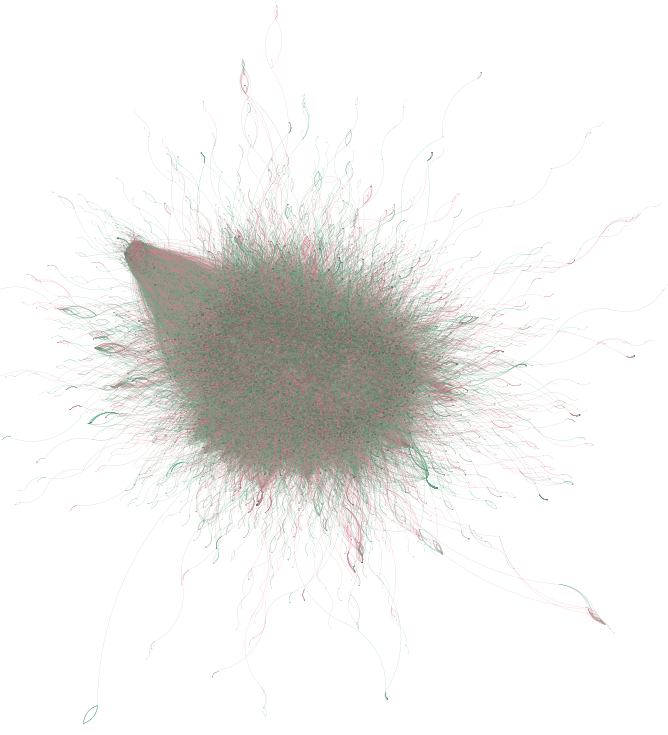
\includegraphics[width=0.8\linewidth]{figures/init_fb.png}
    \caption{Facebook Network}
    \label{fig:enter-label}
\end{figure}

The second network we examined was the Epinions social network \cite{McAuleyLeskovec2012}, which is a directed graph where each node represents a user on the Epinions.com review website, and each edge will either state whether the user trusts or distrusts another user. The network is comprised of 131,828 nodes and 841,372 edges. Although the entire users form a large strong weakly connected component of 119,130 nodes (90.4\% of the graph) with 833,695 edges (99.1\% of the total). The strongly connected component is relatively small, i.e., just 41,441 users (31.4\%) who mutually trust one another with 693,737 edges (82.5\%). The average clustering coefficient of the network is 0.1279, which indicates moderate local clustering. Lastly, this network also has a small-world nature, with the diameter being 14. 

\begin{figure}[ht]
    \centering
    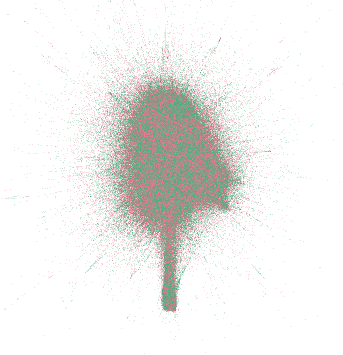
\includegraphics[width=0.8\linewidth]{figures/init_epinions.png}
    \caption{Epinions Network}
    \label{fig:enter-label}
\end{figure}
